\documentclass{article}
\usepackage[utf8]{inputenc}
\usepackage{hyperref}
\usepackage[english]{babel}
\usepackage{latexsym,bm,amsmath,amssymb,graphicx,ctex,tikz,systeme,array, soul,scalerel,wrapfig,lipsum}
\newcommand*\circled[1]{\tikz[baseline=(char.base)]{
            \node[shape=circle,draw,inner sep=2pt] (char) {#1};}}
\usepackage{extarrows}% http://ctan.org/pkg/extarrows
\newcommand*{\vertbar}{\rule[-1ex]{0.5pt}{2.5ex}}
\newcommand*{\horzbar}{\rule[.5ex]{2.5ex}{0.5pt}}
\newcommand{\eqdef}{\xlongequal{\text{def}}}%
\usepackage{geometry}
 \geometry{
 a4paper,
 total={170mm,257mm},
 left=10mm,
 right=10mm,
 top=20mm,
 }
\usepackage{subfig}
\usepackage{wrapfig}
\usepackage{multirow}
\usepackage{multicol}
\usepackage{graphicx}
\usepackage{titling}
\usepackage{listings}
\usepackage{xcolor}
\usepackage[lighttt]{lmodern}
\definecolor{codegreen}{rgb}{0,0.6,0}
\definecolor{codegray}{rgb}{0.5,0.5,0.5}
\definecolor{codepurple}{rgb}{0.58,0,0.82}
\definecolor{backcolour}{rgb}{0.95,0.95,0.92}
\lstdefinestyle{mystyle}{
    backgroundcolor=\color{backcolour},   
    commentstyle=\color{codegreen},
    keywordstyle=\color{magenta},
    numberstyle=\tiny\color{codegray},
    stringstyle=\color{codepurple},
    basicstyle=\sffamily\large,
    breakatwhitespace=false,         
    breaklines=true,                 
    captionpos=b,                    
    keepspaces=true,                 
    numbers=left,                    
    numbersep=5pt,                  
    showspaces=false,                
    showstringspaces=false,
    showtabs=false,                  
    tabsize=2
}

\lstset{style=mystyle}
\newcommand{\subs}[1]{\subsection*{#1}}
\newcommand{\secs}[1]{\section*{#1}}
 
\usepackage{fancyhdr}
\fancypagestyle{plain}{%  the preset of fancyhdr 
    \fancyhf{} % clear all header and footer fields
    \fancyfoot[R]{Guyuan Xu\\224040074}
    \fancyfoot[L]{\thedate}
    \fancyhead[L]{MDS 6106 Optimization and Modeling}
    % \fancyhead[R]{\theauthor}
}
\makeatletter
\def\@maketitle{%
  \newpage
  \null
  \vskip 1em%
  \begin{center}%
  \let \footnote \thanks
    {\LARGE \@title \par}%
    \vskip 1em%
    %{\large \@date}%
  \end{center}%
  \par
  \vskip 1em}
\makeatother

% \usepackage{lipsum}  
% \usepackage{cmbright}



%======================================= document ======================================
%======================================= document ======================================
%======================================= document ======================================

\begin{document}
\title{\raggedright MDS 6106 Assignment 4}
%\author{Guyuan Xu \\224040074}
\date{Nov 20th, 2024}
\maketitle

\noindent\begin{tabular}{@{}ll}
   Guyuan Xu &\href{mailto:224040074@link.cuhk.edu.cn}{224040074} \\
    
%
\end{tabular}


\secs{A4.1 (Implementing the Gradient Method)}
We want to minimize the objective function
\[
\min_{x\in\mathbb{R}^2} f(x) = \frac{1}{2}x_1^4-x_1^3-x_1^2+x_1^2x_2^2+\frac{1}{2}x_2^4-x_2^2
\]
by gradient descent methods with different initial points and stepsize strategies, as presented in the following.\\

\noindent Initial points: 
\[
\chi^0 := \left\{
\begin{bmatrix}
-\frac{1}{2} \\ 1
\end{bmatrix},
\begin{bmatrix}
-\frac{1}{2} \\ \frac{1}{2}
\end{bmatrix},
\begin{bmatrix}
-\frac{1}{4} \\ -\frac{1}{2}
\end{bmatrix},
\begin{bmatrix}
\frac{1}{2} \\ -\frac{1}{2}
\end{bmatrix},
\begin{bmatrix}
\frac{1}{2} \\ 1
\end{bmatrix}
\right\}
\]
\noindent stationary points of $f(x)$:
\[
\chi^* := \left\{
\begin{bmatrix}
0 \\ 0
\end{bmatrix},
\begin{bmatrix}
2 \\ 0
\end{bmatrix},
\begin{bmatrix}
-\frac{1}{2} \\ 0
\end{bmatrix},
\begin{bmatrix}
0 \\ 1
\end{bmatrix},
\begin{bmatrix}
0 \\ -1
\end{bmatrix}
\right\}
\]



%------------ backtracking--------------
\subsection*{1. Backtracking}
\begingroup
\setlength{\intextsep}{0pt}%
\setlength{\columnsep}{0pt}%
\begin{wrapfigure}{r}{0.65\textwidth}%靠文字内容的右侧
  \centering
  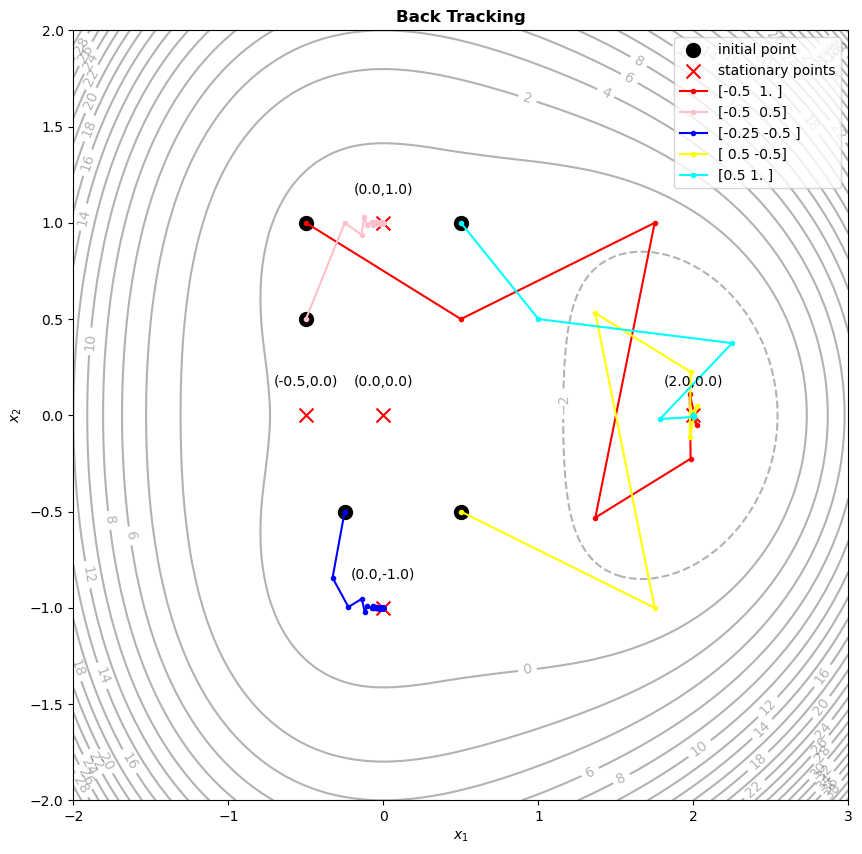
\includegraphics[width=\linewidth]{Back Tracking.png}
  \caption{Backtracking Line Search}
\end{wrapfigure}

Back Tracking line search: choose the largest $\alpha_k \in \{\sigma^k: k = 0,1,...\}$ that satisfies Armijo condition $f(x_k+\alpha_k d_k)-f(x_k)\leq \gamma \alpha_k \nabla f(x_k)^T d_k$ with $(\sigma, \gamma) = (0.5,0.1)$.\\
\\
Performance (in terms of iteration) of Backtracking Line Search stepsize strategy are shown below:\\
\\
  \begin{tabular}{ccc}
    
    \hline
    $x_0$ & iteration & limit point $x^*$\\
    \hline
          (-0.50,1.00) & 13 & (2.00,-0.00)  \\ % backtrack
          (-0.50,0.50) & 325 & (-0.00,1.00) \\ % backtrack
          (-0.25,-0.50) & 467 & (-0.00,-1.00)  \\ % backtrack
          (0.50,-0.50) & 12 & (2.00,0.00)  \\ % backtrack
          (0.50,1.00) & 10 & (2.00,-0.00)  \\ % backtrack
          \hline
          \multicolumn{3}{c}{Backtracking Line Search}\\
          \hline
  \end{tabular}

  \endgroup
\newpage
%------------------ exact line search ----------------------
\subs{2. Exact Line Search}

\begingroup
\setlength{\intextsep}{0pt}%
\setlength{\columnsep}{0pt}%
\begin{wrapfigure}{r}{0.65\textwidth}%靠文字内容的右侧
  \centering
  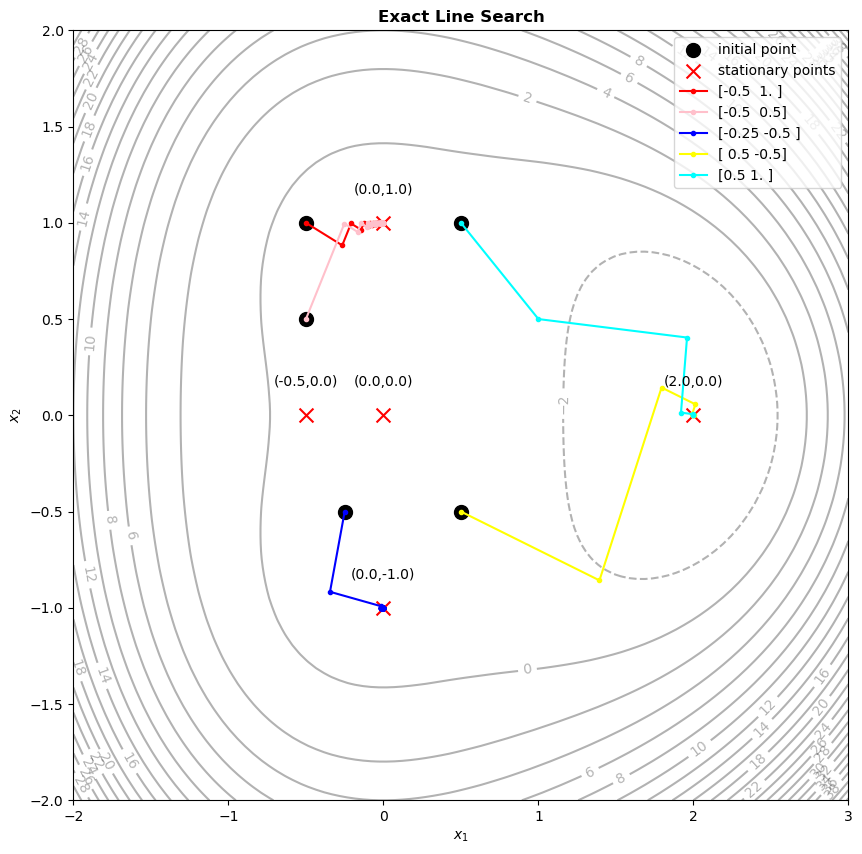
\includegraphics[width=\linewidth]{Exact Line Search.png}
  %\caption{Exact Line Search}
\end{wrapfigure}

Exact Line Search: aim at choosing the stepsize $\alpha_k$ that 
\[
\alpha_k = \underset{\alpha_k \geq 0}{argmin}\; f(x_k+\alpha_k d_k)
\]
Performance of Exact line search stepsize strategy are shown below:\\

\noindent\begin{tabular}{ccc}
    
  \hline
  $x_0$ & iteration & limit point $x^*$\\
  \hline
  (-0.50,1.00) & 295 & (-0.00,1.00)   \\ % exactlineS
  (-0.50,0.50) & 296 & (-0.00,1.00)  \\ % exactlineS
  (-0.25,-0.50) & 375 & (-0.00,-1.00)  \\ % exactlineS
  (0.50,-0.50) & 9 & (2.00,0.00) \\ % exactlineS
  (0.50,1.00) & 6 & (2.00,0.00)  \\ % exactlineS
        \hline
        \multicolumn{3}{c}{Exact Line Search}\\
        \hline
\end{tabular}\\
\\
\textbf{\# PS}: the paths of 2 consecutive steps are not perpendicular because we constraint $\alpha_k \leq 1$ (because we search $\alpha$ in $[0,a]$, where $a=1$) insetead of not setting any constraint to them.

\endgroup
\vspace{1cm}

%------------- diminishing -----------------
\subs{3. Diminishing Stepsize}

\begingroup
\setlength{\intextsep}{0pt}%
\setlength{\columnsep}{0pt}%
\begin{wrapfigure}{r}{0.65\textwidth}%靠文字内容的右侧
  \centering
  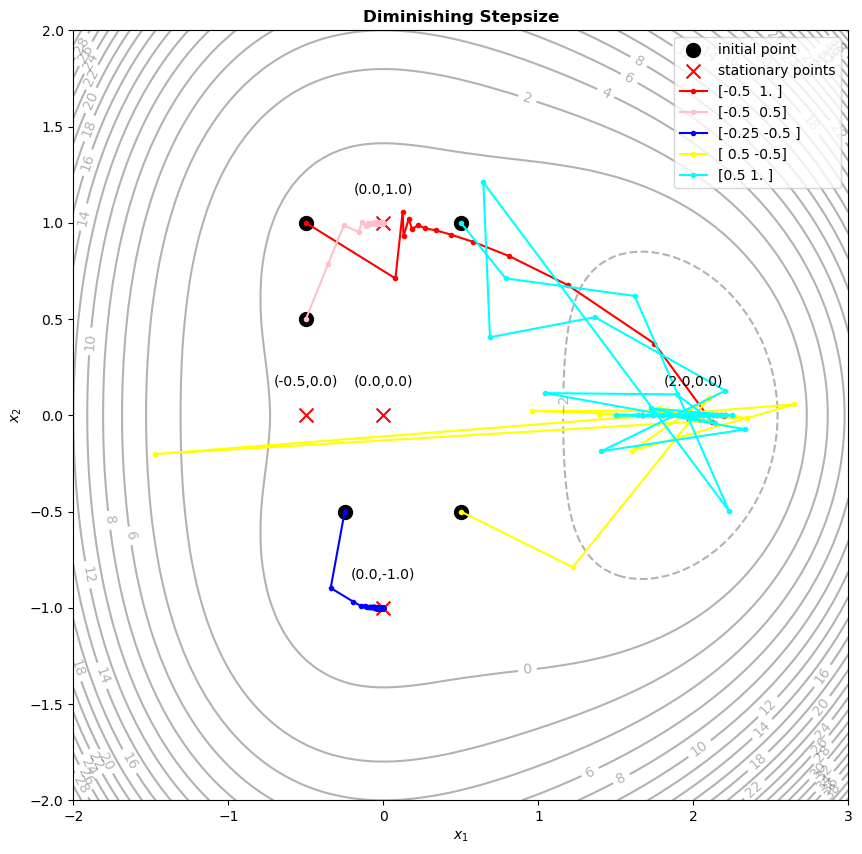
\includegraphics[width=\linewidth]{Diminishing Stepsize.png}
  %\caption{Diminishing Stepsize}
\end{wrapfigure}

\noindent Diminishing Stepsize: we simply set
\[
  \alpha_k = \frac{1}{\sqrt{k+2}}
\]
where $k$ is the round of iteration.\\
Performance of diminishing stepsize strategy are shown below:

\noindent\begin{tabular}{ccc}
    
  \hline
  $x_0$ & iteration & limit point $x^*$\\
  \hline
  (-0.50,1.00) & 47 & (2.00,0.00)  \\ % diminishing
  (-0.50,0.50) & 8523 & (-0.00,1.00) \\ % diminishing
  (-0.25,-0.50) & 8501 & (-0.00,-1.00)  \\ % diminishing
  (0.50,-0.50) & 47 & (2.00,-0.00)  \\ % diminishing
  (0.50,1.00) & 47 & (2.00,0.00)  \\ % diminishing
        \hline
        \multicolumn{3}{c}{Diminishing Stepsize}\\
        \hline
\end{tabular}\\
\\
\textbf{\# PS}: Since HW sheet has no requirement on $k$, we follow the common sense that $k$ starts from 1, so the first stepsize is
\[
  \alpha_1 = \frac{1}{\sqrt{1+2}} = \frac{1}{\sqrt{3}} 
\]

\endgroup

\newpage
%------------- conclusion of stepsize strategy ---------------
Then we can conclude the performance of different stepsize strategies as the following table:

  \begin{center}
    \begin{tabular}{|c|cccc|} 
        \hline
        Methods & $x_0$ & iteration & limit point $x^*$ & Global Minimum?\\
        \hline
        &(-0.50,1.00) & 13 & (2.00,-0.00) & yes\\ % backtrack
        &(-0.50,0.50) & 325 & (-0.00,1.00) & no \\ % backtrack
        Back Tracking&(-0.25,-0.50) & 467 & (-0.00,-1.00) & no \\ % backtrack
        &(0.50,-0.50) & 12 & (2.00,0.00) & yes \\ % backtrack
        &(0.50,1.00) & 10 & (2.00,-0.00) & yes \\ % backtrack
        \hline
        \hline
        &(-0.50,1.00) & 295 & (-0.00,1.00) & no \\ % exactlineS
        &(-0.50,0.50) & 296 & (-0.00,1.00) & no \\ % exactlineS
        Exact Line Search&(-0.25,-0.50) & 375 & (-0.00,-1.00) & no \\ % exactlineS
        &(0.50,-0.50) & 9 & (2.00,0.00) & yes \\ % exactlineS
        &(0.50,1.00) & 6 & (2.00,0.00) & yes \\ % exactlineS
        \hline
        \hline
        &(-0.50,1.00) & 47 & (2.00,0.00) & yes\\ % diminishing
        &(-0.50,0.50) & 8523 & (-0.00,1.00) & no \\ % diminishing
        Diminishing Stepsize&(-0.25,-0.50) & 8501 & (-0.00,-1.00) & no \\ % diminishing
        &(0.50,-0.50) & 47 & (2.00,-0.00) & yes\\ % diminishing
        &(0.50,1.00) & 47 & (2.00,0.00) & yes \\ % diminishing
      \hline
    \end{tabular} 
\end{center}
\newpage

\secs{A4.2 (Inertial Gradient Method)}

\noindent The convergence trace of gradient method with momentum of $\beta \in \{0.3,0.5,0.7,0.9\}$ and different initial points are shown below respectively:\\
\vspace{5mm}

\noindent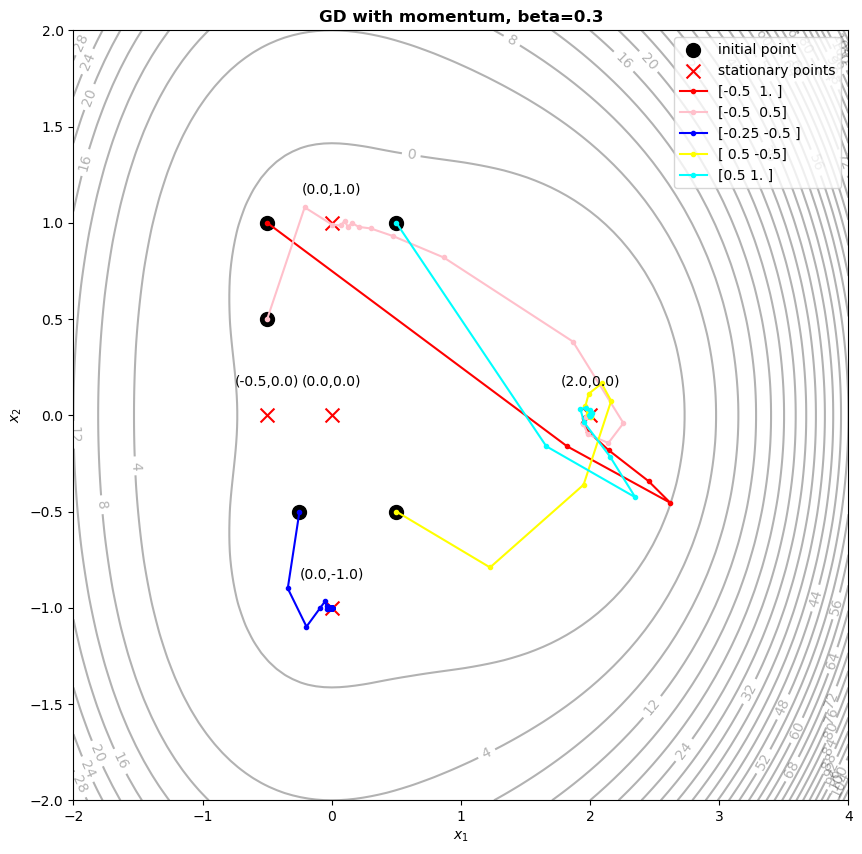
\includegraphics[width=0.5\linewidth]{GD with momentum, beta=03.png}
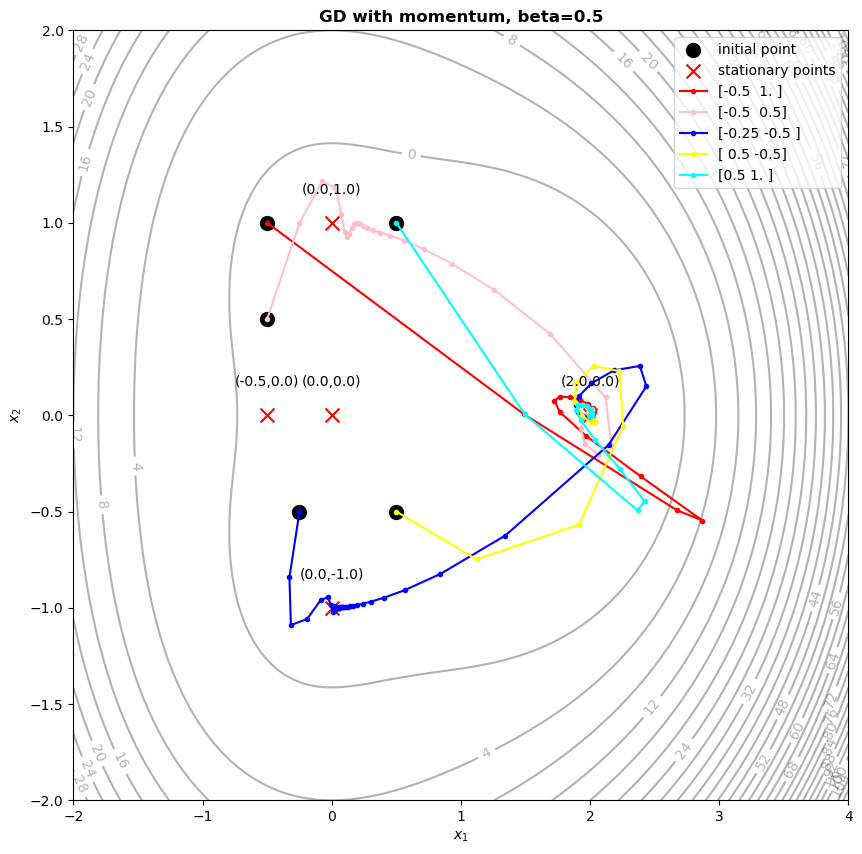
\includegraphics[width=0.5\linewidth]{GD with momentum, beta=05.png}\\
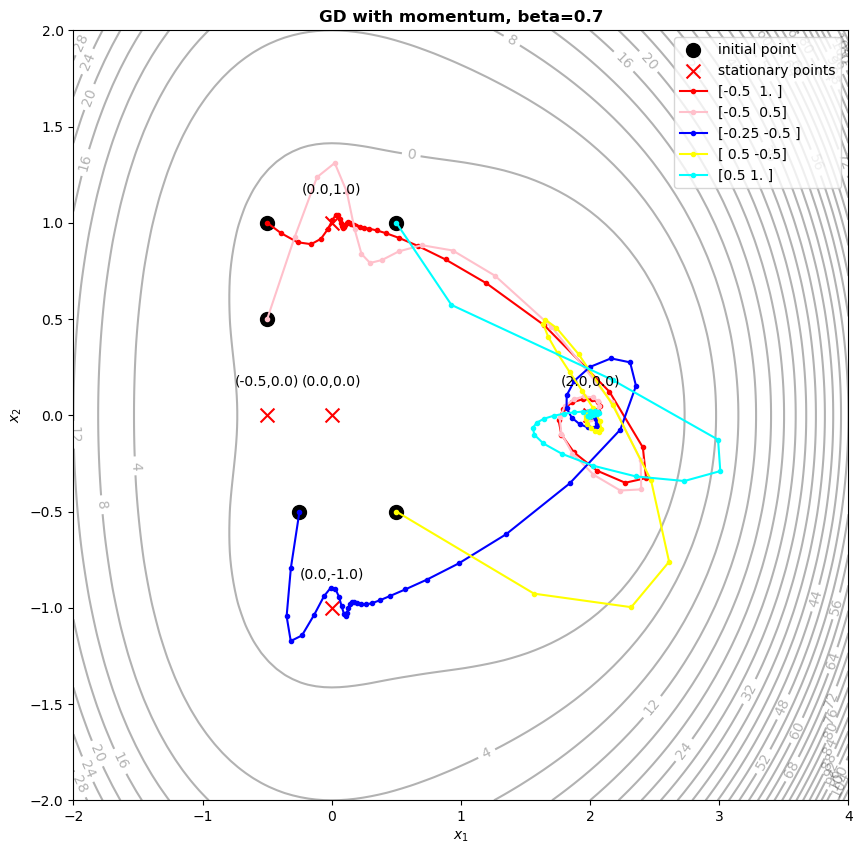
\includegraphics[width=0.5\linewidth]{GD with momentum, beta=07.png}
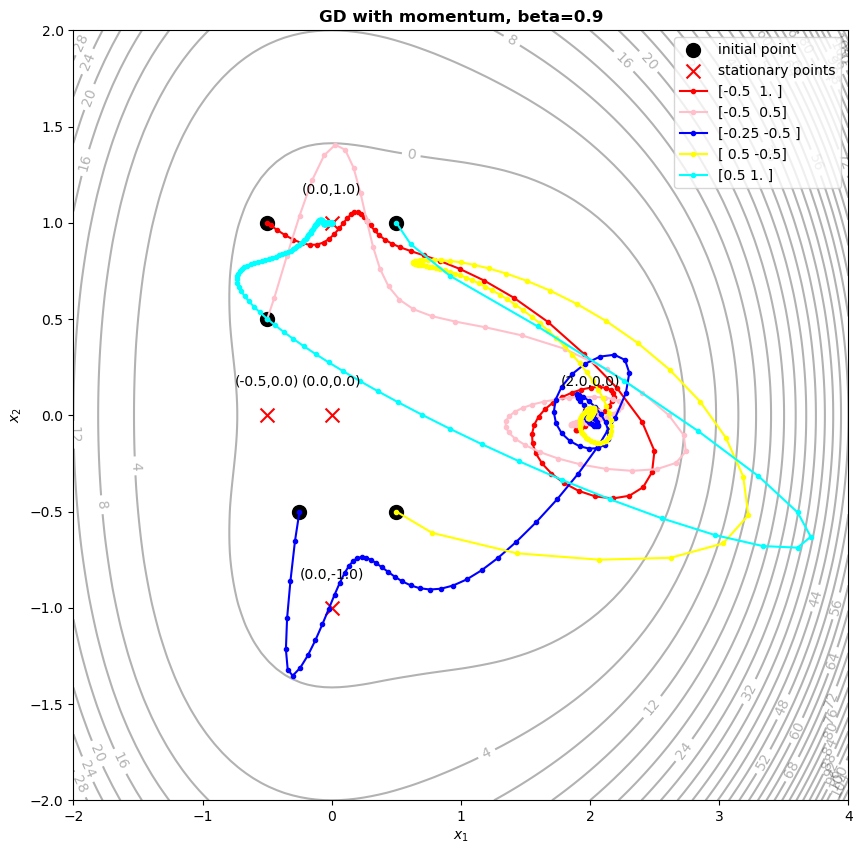
\includegraphics[width=0.5\linewidth]{GD with momentum, beta=09.png}\\

\subs{Performance Analysis}
by comparing the average iteration numbers of GD with momentum and GD with different stepsize strategies (discussed in part A4.1):
\begin{center}
  \begin{tabular}{c|ccc|cccc}
    \hline
    \multicolumn{1}{c}{} & \multicolumn{3}{c}{Stepsize strategies} & \multicolumn{4}{c}{GD with momentum}\\
    \hline
    &Backtrack & Exact LineSearch & Diminishing & $\beta = 0.3$ & $\beta = 0.5$ & $\beta = 0.7$ & $\beta = 0.9$\\
    \hline
    Average Iteration & 164.5 & 196.2 & 3433.0 & 104.8& 51.8 & 90.2 & 1250.0\\
    \hline
    Probablity to Global Min & 0.6 & 0.4 & 0.6 & 0.8 & 1.0 & 1.0 &0.8\\
    \hline
  \end{tabular}
\end{center}
It is easy to see that \textbf{the average iteration (averaging across 5 different initial points) it takes to converge to some limit point is noticeably larger using stepsize strategies than GD with momentum in general.}  \\
\\
And we also notice GD with momentum converger faster when $\beta$ change from $0.3$ to $0.5$, then converger slower when $\beta$ goes from $0.5$ to $0.9$, how to interpretate this phenomenon? we can first look at the detail of how $\beta$ affect convergence: 

\begin{center}
  \begin{tabular}{|c|cccc|} 
      \hline
      $\beta$ & $x_0$ & iteration & limit point $x^*$ & Global Minimum? \\
      \hline
      &(-0.50,1.00) & 26 & (2.00,0.00) & yes\\ % momentum beta 0.3
      &(-0.50,0.50) & 33 & (2.00,-0.00) & yes \\ % momentum beta 0.3
      $\beta = 0.3$&\textcolor{red}{(-0.25,-0.50)} & \textcolor{red}{417} & \textcolor{red}{(-0.00,-1.00)} & no \\ % momentum beta 0.3
      &(0.50,-0.50) & 24 & (2.00,0.00) & yes \\ % momentum beta 0.3
      &(0.50,1.00) & 24 & (2.00,0.00) & yes \\ % momentum beta 0.3
      \hline
      \hline
      &(-0.50,1.00) & 39 & (2.00,0.00) & yes \\ % momentum beta 0.5
      &(-0.50,0.50) & 56 & (2.00,0.00) & yes \\ % momentum beta 0.5
      $\beta = 0.5$&(-0.25,-0.50) & 88 & (2.00,0.00) & yes \\ % momentum beta 0.5
      &(0.50,-0.50) & 37 & (2.00,-0.00) & yes \\ % momentum beta 0.5
      &(0.50,1.00) & 39 & (2.00,0.00) & yes \\ % momentum beta 0.5
      \hline
      \hline
      &(-0.50,1.00) & 105 & (2.00,0.00) & yes \\ % momentum beta 0.7
      &(-0.50,0.50) & 88 & (2.00,0.00) & yes \\ % momentum beta 0.7
      $\beta = 0.7$&(-0.25,-0.50) & 102 & (2.00,-0.00) & yes \\ % momentum beta 0.7
      &(0.50,-0.50) & 77 & (2.00,-0.00) & yes \\ % momentum beta 0.7
      &(0.50,1.00) & 79 & (2.00,-0.00) & yes \\ % momentum beta 0.7
    \hline
    \hline
    &(-0.50,1.00) & 268 & (2.00,0.00) & yes \\ % momentum beta 0.9
    &(-0.50,0.50)& 258 & (2.00,0.00) & yes \\ % momentum beta 0.9
    $\beta = 0.9$&(-0.25,-0.50) & 276 & (2.00,0.00) & yes \\ % momentum beta 0.9
    &(0.50,-0.50) & 297 & (2.00,-0.00) & yes \\ % momentum beta 0.9
    &\textcolor{red}{(0.50,1.00)} & \textcolor{red}{5151} & \textcolor{red}{(-0.00,1.00)} & no \\ % momentum beta 0.9
    \hline
  \end{tabular} 
\end{center}
Notice when $\beta = 0.3$ and starting from the initial point $(-0.25,-0.5)$, GD converge to $(0,-1)$ while other initial points all converge to $(2,0)$, this is because the first several stepsize of GD heppen to be too large from this initial point and \textbf{pushing the trace to an area not ideal for fast convergence}, and by coincidence the trace finally converge to a different limit point from the other initial points, and the iterations it takes to converge go very high, this should \textbf{be treated as an anomoly.} Same with $\beta = 0.9$ initial point $(0.5,1.0)$: this very initial condition just happen to be not ideal for fast convergence.\\
After dropping this anomoly we can get an averge iteration number of $26.75$ for $\beta = 0.3$, and the trend becomes obvious: $\beta$ smaller, converge faster. \\
\\
Another observation is that \textbf{GD with momentum is more likely to converge to the global minimum} $(2,0)$ than GD with stepsize strategies, this is also easy to explain: with "momentum" (brought by the momentum term $\beta (x_k-k_{k-1})$), the trace is more likely to "escape" from the local minimum.
\newpage





\end{document}


